


\documentclass[11pt]{book}
\usepackage[paperwidth=17cm, paperheight=22.5cm, bottom=2.5cm, right=2.5cm]{geometry}
\usepackage{amssymb,amsmath,amsthm} %paquete para símbolo matemáticos
\usepackage[spanish]{babel}
\usepackage[utf8]{inputenc} %Paquete para escribir acentos y otros símbolos directamente
\usepackage{enumerate}
\usepackage{graphicx}
\usepackage{caption}
\usepackage{subcaption}
\graphicspath{{Img/}} %En qué carpeta están las imágenes
\usepackage[nottoc]{tocbibind}
\usepackage[pdftex,
            pdfauthor={GREGORIO INIESTA OVEJERO},
            pdftitle={Investigación, evaluación e implementación de métodos que simulen seis grados de libertad en fotos y vídeo para Realidad Virtual},
            pdfsubject={Fotos y vídeo en realidad virtual},
            pdfkeywords={6DOF, Foto, Video, Realidad Virtual},
            pdfproducer={Latex con hyperref},
            pdfcreator={pdflatex}]{hyperref}

\usepackage{beton}
\usepackage{euler}
\usepackage[rm]{roboto}
\usepackage[T1]{fontenc}

\renewcommand{\familydefault}{\sfdefault}

%-----------
%	TITLES REFORMAT
%-----------

\usepackage{titlesec}
\titleformat{\chapter}{\bfseries\Large}{\arabic{chapter}.~}{0pt}{}

\begin{document}

\title{TFM - FOTOS Y VÍDEO 6DOF} %Con este nombre se guardará el proyecto en writeLaTex


\begin{titlepage}
\begin{center}

\begin{figure}[h]
\centering
\begin{subfigure}{.5\textwidth}
	\centering
	
\includegraphics[width=0.9\linewidth]{logo_ucjc.png}
\end{subfigure}%
\begin{subfigure}{.5\textwidth}
	\centering
	
\includegraphics[width=0.9\linewidth]{logo-u-tad.jpg}
\end{subfigure}
\end{figure}


\vspace{4em}

\textsc{\Huge \textmd{Máster en Computación Gráfica y Simulación}}
\\[3em]

{\LARGE 2018}
\\[3em]

{\large Trabajo de Final de Máster}
\\[3em]

\begin{tabular}{ p{0.85\textwidth} }
\centering
{\Large Investigación, evaluación e implementación de métodos que simulen seis grados de libertad en fotos y vídeo para Realidad Virtual}
\end{tabular}

\vspace{6em}

\begin{tabular}{ l l }
	\textbf{Autor:} & Gregorio Iniesta Ovejero \\
	\textbf{Tutor:} & Diego Bezares Sánchez
\end{tabular}


\end{center}

\vspace*{\fill}

\end{titlepage}


%----------------------------------------------------------------------------------------
%	INDICE
%---------------------------------------------------------------------------------------

\tableofcontents

%----------------------------------------------------------------------------------------
%	SECCIONES
%----------------------------------------------------------------------------------------
\mainmatter %empieza la numeración de las páginas
\pagestyle{headings}

%  Incluye los capítulos en el folder de capítulos

%RESUMEN (1 hoja)
%----------------------------------------------------------------------------------------
%	RESUMEN (1 hoja)
%----------------------------------------------------------------------------------------

\pagestyle{empty}
\chapter {Resumen}

El vídeo y la fotografía es, hoy en día, una parte imprescindible del entretenimiento en  realidad virtual, pero tiene grandes desventajas frente a otras tecnologías, como las experiencias en entornos tridimensionales, debido a la falta de interactividad.

Desde hace unos años empresas como Disney, Facebook y Google han establecido un precedente en la industria tecnológica, buscando establecer los llamados seis grados de libertad al vídeo y la fotografía 360º para mejorar la sensación de inmersión. Existen numerosas maneras de conseguir este objetivo y cada una tiene sus ventajas y sus inconvenientes.

El propósito del trabajo descrito en esta memoria es implementar, de la manera más realista y eficiente posible, un sistema que proporcione seis grados de libertad en un rango de movimiento limitado. Para ello se va a recurrir a un algoritmo basado en desplazamientos pixel a pixel, teniendo capacidad de manipulación de la información al nivel mas detallado disponible, haciendo uso de todos los recursos disponibles en los dispositivos incluyendo hardware gráfico con propósito general.

La forma de conseguir este objetivo será evaluar muchas implementaciones para, más tarde, seleccionar los mejores resultados y trabajar sobre ellos con la finalidad de hacerlos más eficientes y realistas. Todo esto sin dejar de contemplar más opciones como las que han implementado otros desarrolladores.

%INTRODUCCIÓN (2,3 hojas)
%----------------------------------------------------------------------------------------
%	INTRODUCCIÓN (2,3 hojas)
%----------------------------------------------------------------------------------------

% Actualmente la realidad virtual tiene una variedad muy grande de dispositivos con diferentes características. Las principales especificaciones a tener en cuenta a la hora de decidir utilizar uno en concreto son la disponibilidad de accesorios como los mandos, la resolución de pantalla y los grados de libertad tanto de las gafas como de los periféricos, siendo típicos 3 y 6 grados.
% https://twitter.com/Diegobez/status/1038067397201207296
% https://twitter.com/Diegobez/status/925033415442919424








\pagestyle{empty}
\chapter{Introducción}
% tema de trabajo
La realidad virtual es una tecnología que desde hace unos años ha estado intentando hacerse un hueco en la industria del entretenimiento. Unity expuso estadísticas de consumo de realidad virtual durante el pasado año, proporcionando cifras como un 134\% de crecimiento en sobremesa y consola y un 295\% de crecimiento en las instalaciones de realidad virtual en móvil lo que hace casi un millón de usuarios activos en aplicaciones hechas con Unity a finales de 2017. Por último las estadisticas de uso en multimedia superan el 50\% del tiempo de uso llegando a más del 80\% según Facebook \cite{FBOculusGo}.

\begin{figure}[h]
\centering
\begin{subfigure}{.5\linewidth}
	\centering
	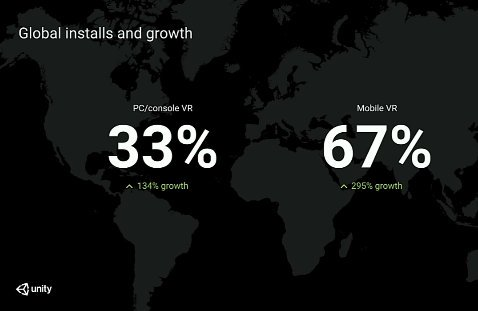
\includegraphics[width=0.93\linewidth]{Unite/global-installs.jpg}
\end{subfigure}%
\begin{subfigure}{.5\linewidth}
	\centering
	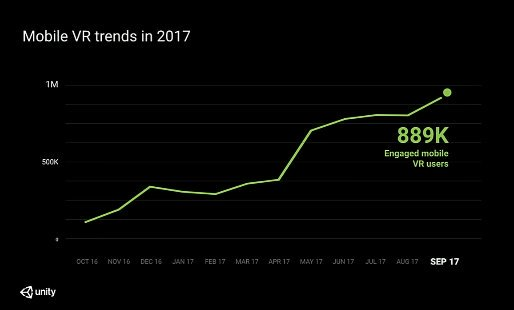
\includegraphics[width=\linewidth]{Unite/mobile-trends.jpg}
\end{subfigure}
\end{figure}


\section{Grados de libertad}
Un factor clave a tener en cuenta cuando hablamos de realidad virtual son los grados de libertad, que definen la capacidad de movimiento a la hora de interactuar. Generalmente se habla de tres y seis grados de libertad. En el caso de tres grados de libertad, hace referencia a los giros sobre el eje principal (viraje o \textit{yaw}, inclinación o \textit{pitch} y cabeceo o \textit{roll}), mientras que cuando se amplia a seis grados de libertad hace referencia al desplazamiento en los tres ejes. Esto aplicado a las gafas de realidad virtual informa de la capacidad del dispositivo de captar los giros de la cabeza en todas las direcciones (tres grados de libertad) o si además capta el desplazamiento por la sala (seis grados de libertad).

El mercado de dispositivos de realidad virtual se está enfocando hacia seis grados de libertad. La alta gama ya dispone de ellos desde el principio mientras la gama media y baja ya está adaptándose como demuestra Oculus Santa Cruz o Vive Focus.

\section{Foto y vídeo en realidad virtual}
El contenido que se genera todavía esta basado en gran parte en técnicas ya conocidas como reproducción de vídeo y fotos cuya máxima adaptación consiste simplemente en poner una imagen ligeramente diferente en cada ojo.

La característica principal de este tipo de contenido es que cada imagen esta tomada desde un punto fijo en el espacio. Esto provoca una problemática que consiste en que el usuario únicamente tiene tres grados de libertad a la hora de visualizarlo en unas gafas de realidad virtual. Además de esta restricción debido a las técnicas de grabación que se usan, el cabeceo o \textit{roll} provoca ver imágenes duplicadas y puede provocar incomodidad o incluso mareo.

Debido a las estadísticas de consumo del contenido multimedia grandes empresas como Google, Facebook y Disney entre otras, están trabajando en mejorar los sistemas de visualización de vídeo y fotos mediante vídeo volumétrico, campos de luz o fotogrametría.

%La mayoría de proyectos que están disponibles actualmente utilizan técnicas que transforman cada frame en polígonos y desplazan los vértices en función de la profundidad que le indica un mapa de profundidad. Esto provoca en demasiadas ocasiones una deformación de elementos pequeños y en algunas ocasiones se ocultan elementos que deberían ser visibles de otro modo.

\section{Qué aporta este proyecto}
%que aporta que aporta
Este trabajo toma la demo ``Welcome to lightfields'' como referencia pero creando un proyecto de código libre. Trata de conseguir una sensación real de tres dimensiones habilitando seis grados de libertad en un espacio reducido de desplazamiento a partir de un vídeo estereoscópico plano en dos dimensiones y su mapa de profundidad. Para ello se hará un paralaje en tres dimensiones píxel a píxel en función del mapa de profundidad y la posición del usuario.

Durante el desarrollo del proyecto se llevan a cabo pruebas con diferentes técnicas y se evalúa la viabilidad en diferentes dispositivos (plataformas móviles y de sobremesa), el realismo del resultado así como la escalabilidad de los métodos.
















% interés
% Consumo de contenido
% Las gafas van a 6dof
% Hay gente que esta trabajando en ello (Facebook, Google)

%PLANTEAMIENTO DEL PROBLEMA (1 hoja)
%----------------------------------------------------------------------------------------
%	PLANTEAMIENTO DEL PROBLEMA (1 hoja)
%----------------------------------------------------------------------------------------

\pagestyle{empty}
\chapter {Planteamiento del problema}

La fotografía y el vídeo para realidad virtual actualmente tienen muchas limitaciones tanto para producirlo como para visualizarlo. Una de estas limitaciones y del cual este proyecto se ocupa es la falta de libertad movimiento. 

La foto y el vídeo sólo tienen tres grados de libertad y de ellos cabeceo o \textit{roll} (inclinar la cabeza sobre los hombros) no funciona como cabría esperar y puede provocar desde mareos hasta ver las imágenes duplicadas. La captura de imágenes tanto reales como virtuales se hace con cámaras que irremediablemente están en un punto concreto del espacio y eso en principio limita el movimiento del usuario.

En mayo de 2017, Google dio una charla aportando que cerca del 50\% del tiempo pasado en Daydream se centra en experiencias de vídeo. Un año después Facebook en el F8 \cite{FBOculusGo}, hablando sobre el estudio para el diseño de Oculus Go, puso de manifiesto que el 99\% de los usuarios consumen vídeo y que el 83\% de tiempo utilizado se destina a multimedia llegando a la conclusión que es uno de los casos de uso principales.

Por ello, este trabajo se centra en mejorar la visualización del vídeo con un sistema que permita al usuario desplazarse físicamente dentro de un área reaccionando el vídeo a ese posicionamiento en tiempo real.

%OBJETIVOS (1 hoja)
%----------------------------------------------------------------------------------------
%	OBJETIVOS (1 hoja)
%----------------------------------------------------------------------------------------

\pagestyle{empty}
\chapter {Objetivos}

Este proyecto ha sido creado con el objetivo de investigar, evaluar e implementar software para proporcionar seis grados de libertad en la visualización de contenidos a partir de imágenes planas y su mapa de profundidad aplicado en tecnologías de realidad virtual.

%ESTADO DEL ARTE (20-25 hojas)
%----------------------------------------------------------------------------------------
%	ESTADO DEL ARTE (20-25 hojas)
%----------------------------------------------------------------------------------------

\pagestyle{empty}
\chapter {Estado del Arte}

La acepción de realidad virtual que va a ser tratado en este trabajo es un mundo generado por ordenador. Se puede interactuar con este mundo por medio diferentes dispositivos como los hápticos o los olfativos, pero la forma más común actualmente y en la cual se va a centrar este documento es en la representación de imágenes mediante un casco o gafas de realidad virtual.

\section{Marco teórico}

\subsection{Fotografía y vídeo}
La fotografía y el vídeo en realidad virtual es un campo muy amplio en el que se pueden encontrar diferentes maneras guardar y reproducir la información. A continuación se comentan algunos conceptos importantes para entender el resto del documento. 

\textbf{Nota:} Están organizados por conceptos alternativos, es decir, una foto no puede ser estereoscópica y monoscópica al mismo tiempo.

\subsubsection{Estereoscopía/Monoscopía}
La monoscopía implica que sólo existe una imagen para ambos ojos y por lo tanto no hay sensación de profundidad.

La estereoscopía es un factor muy importante en contenido multimedia para realidad virtual puesto que es el que más favorece la inmersión, como se explica en \cite{DiegoBezStereoscopy}. Consiste en tener dos imágenes que muestran la misma escena desde dos puntos cercanos a una distancia fija (normalmente de 6,5cm) y que representan la posición de los ojos (\ref{fig:stereo-example}). Cada una de estas imágenes se reproducen en una de las pantallas de las gafas, de tal manera que el cerebro del usuario se encarga de reconstruir la escena como si fuera realmente tridimensional. Aunque exista la ilusión de tridimensionalidad no es posible desplazarse por el entorno capturado.

\begin{figure}[H]
  \centering
  \includegraphics[width=\textwidth]{stereo-example}
  \caption{Ejemplo de imagen estéreo con lineas verticales para poder comparar el desplazamiento.}
  \label{fig:stereo-example}
\end{figure}
\FloatBarrier

Es importante tener en cuenta que la separación entre las cámaras definirá la sensación de tamaño. Nuestro cerebro interpreta que si las cámaras están a menos distancia que nuestros ojos, todo es más grande y será mas pequeño si ponemos demasiada distancia.

Por último dentro de la estereoscopía se pueden encontrar las distribuciones arriba/abajo o \textit{top/bottom}(\ref{fig:top-bottom-example}) y izquierda/derecha o \textit{side by side}(\ref{fig:side-by-side-example}) que sitúa las imágenes de ojo derecho e izquierdo en vertical u horizontal respectivamente siendo la más extendida \textit{top/bottom}.

\begin{figure}[H]
  \centering
  \includegraphics[width=0.8\textwidth]{top-down}
  \caption{Ejemplo de \textit{top/down}.}
  \label{fig:top-bottom-example}
\end{figure}

\begin{figure}[H]
  \centering
  \includegraphics[width=0.8\textwidth]{side-by-side}
  \caption{Ejemplo de \textit{side by side}.}
  \label{fig:side-by-side-example}
\end{figure}
\FloatBarrier

\subsubsection{Campo de visión}
Por lo general se utilizan dos ángulos para el campo de visión. 

El más conocido y del que se suele hablar trata 360º de visión, es decir, una foto que genera una esfera alrededor de la vista del usuario. Es el que proporciona más inmersión.

El otro ángulo más utilizado es 180º que proporciona toda la visión frontal pero no hay imagen detrás. Las ventajas que más destacan son que puede ser grabado con cámaras poco especializadas y que se puede concentrar mayor cantidad de píxeles en el frente, consiguiendo mayor calidad en la acción destacada.

Existen diferentes métodos para la captura de vídeo como se explicará más adelante.

\subsubsection{Proyecciones}
Una proyección es una forma de representación de un elemento tridimensional, en este caso una geometría esférica, en un espacio bidimensional. A la hora de guardar o reproducir un contenido multimedia es importante tener en cuenta la proyección a utilizar ya que pueden distorisionar la imagen y saturar regiones poco interesantes, como veremos a continuación, con una gran cantidad de píxeles. 

Una de las proyecciones más extendidas y utilizadas en realidad virtual es la equirectangular (\ref{fig:equirect360-example} y \ref{fig:equirect360-schema}), que coincide con la proyección más utilizada en la actualidad para representar el mundo en dos dimensiones. Esta proyección proporciona demasiada información en los polos y que típicamente es el lugar al que menos se suele mirar. Esto hace que gran parte de los píxeles se malgasten. 

Facebook en \cite{FBDynamicStreamming}  propone varias mejoras para su sistema de streamming de vídeo en realidad virtual 360º. Algunas de estas mejoras pueden ser utilizadas también en vídeo local como por ejemplo aplicar una distorsión intencionada a la imagen proporcionando más espacio a la parte central de la imagen y compensando esa distorsión en el reproductor y así obtener más definición en las zonas importantes.

\begin{figure}[H]
  \centering
  \includegraphics[width=\textwidth]{equirect360}
  \caption{Ejemplo de una proyección equirectangular.}
  \label{fig:equirect360-example}
\end{figure}

\begin{figure}[H]
  \centering
  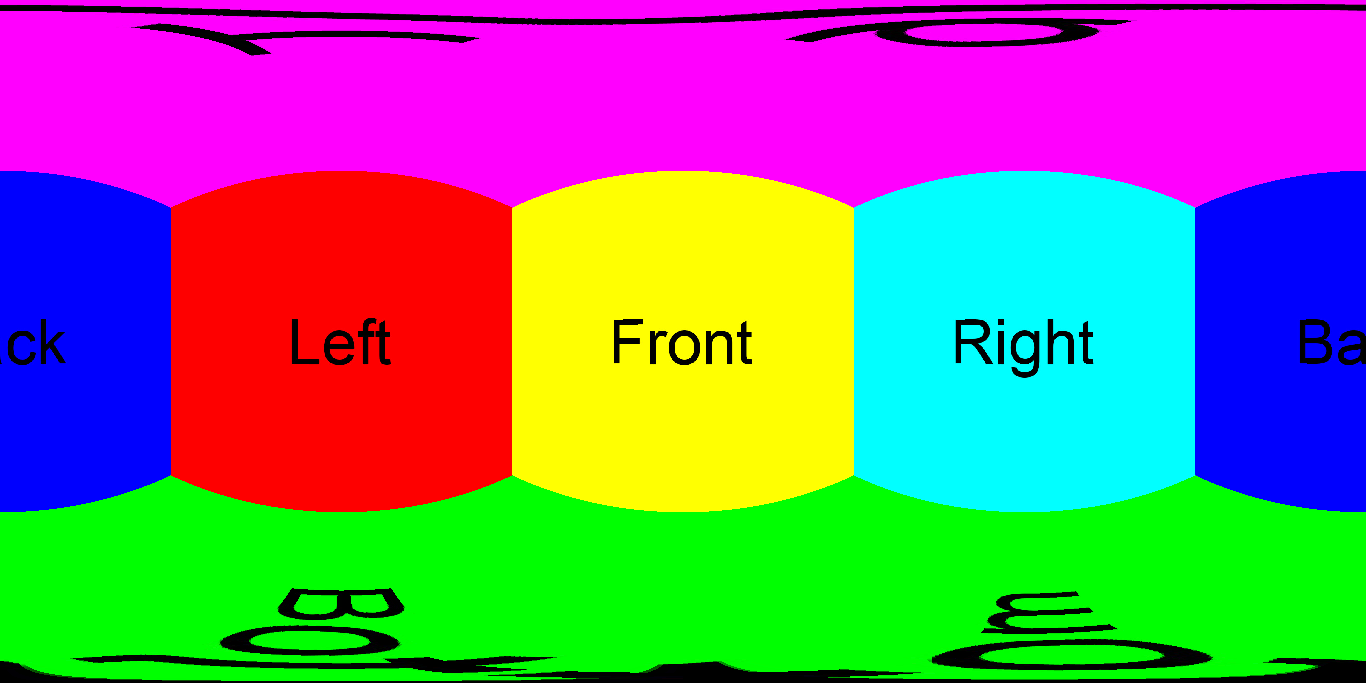
\includegraphics[width=\textwidth]{equirect360-schema}
  \caption{Esquema de una proyección equirectangular.}
  \label{fig:equirect360-schema}
\end{figure}
\FloatBarrier

Otra proyección que se utiliza menos es la cúbica que divide la imagen en seis partes que forman las caras de un cubo. Tiene mayor densidad en las aristas del cubo pero el porcentaje de píxeles útiles aumenta. Normalmente se le aplica una deformación al cubo dándole curvatura reduciendo la densidad de píxeles para que la distribución se más uniforme.

\begin{figure}[H]
  \centering
  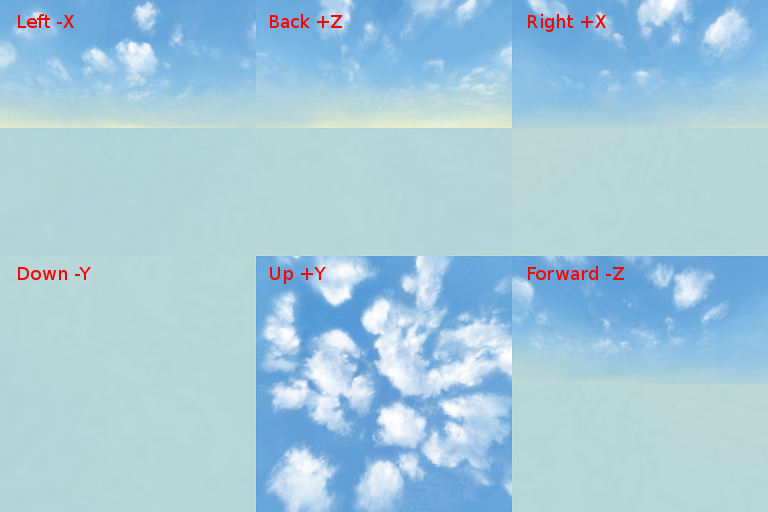
\includegraphics[width=\textwidth]{cubemap}
  \caption{Ejemplo de proyección cúbica.}
  \label{fig:cubemap-example}
\end{figure}
\FloatBarrier

Por último mencionar la proyección de barril que se construye como un cilindro. La distribución de píxeles es uniforme en el campo de visión típico. Esta proyección desaprovecha píxeles que se pierden en los huecos que dejan las tapas del cilindro.

Existen una infinidad de proyecciones y cada una tiene una serie de ventajas e inconvenientes.
 
\subsubsection{Omni-directional Stereo}
La captura con cámara de imágenes estereoscópicas 360º no es trivial.. Existen varios métodos para conseguir esto, y en vídeo el más común consiste en capturar un fotograma en diferentes puntos de una circunferencia teniendo en cuenta el radio de la cabeza, después esas fotos se unen y se reconstruye la imágen. Este proceso es complicado y si no se hace bien, se produce un efecto en el ensambrado llamado stitching y que se evidencia con unos saltos de color o cortes en objetos. Este problema no es trivial y cuesta eliminarlo como se comenta en \cite{DiegoBezStitching}.

Disney y Google proponen un sistema para captura de imágenes llamado ODS (Omni-directional stereo) que explican detalladamente en \cite{GoogleStereoscopy} y \cite{DisneyOmnistereoscopic}. Este sistema consiste en dos cámaras, posicionadas a la distancia ocular y puestas en una circunferencia de un radio similar al de una cabeza. Durante la captura, las cámaras dan una vuelta por la circunferencia y guarda una linea de píxeles por cada posición de la cámara. Esto tiene como consecuencia que únicamente exista una linea de píxeles correcta en cada posición como se puede ver en la figura \ref{fig:ods-schema}.  conlleva implicaciones como que los objetos en la visión periférica no se visualizan correctamente. Pese a esto, la sensación que se consigue es buena y proporciona una gran inmersión.


Por último comentar que el vídeo 180º tiene como beneficio que no necesita de ningún sistema como ODS ya que se hace directamente con cámara sin recurrir a métodos adicionales. Esto hace que todo el area de visualización sea correcta como se muestra en la figura \ref{fig:correct-vision-schema}.


\begin{figure}[H]
\centering
\begin{subfigure}{.40\linewidth}
	\centering
  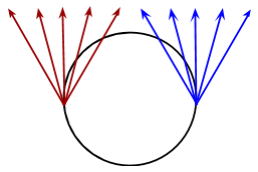
\includegraphics[width=\textwidth]{correct-vision}
  \caption{Esquema de la visión completa.}
  \label{fig:correct-vision-schema}
\end{subfigure}%
\hspace{.05\linewidth}
\begin{subfigure}{.40\linewidth}
	\centering
  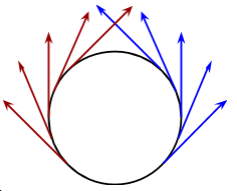
\includegraphics[width=\textwidth]{ods}
  \caption{Esquema de la aproximación hecha con ODS.}
  \label{fig:ods-schema}
\end{subfigure}
\caption{Imágenes obtenidas de \cite{GoogleStereoscopy}.}
\end{figure}

\FloatBarrier

\subsection{Mapas de profundidad}
Debido a la cantidad de técnicas que utilizan mapas de profundidad o \textit{depthmap} es interesante explicar en que consisten. 

Los mapas de profundidad son imagenes que en cada pixel se encuentra codificada la profundidad de la foto en ese punto. Generalmente se utiliza una escala de grises o de rojos aunque se pueden recurrir a métodos más complejos.\cite{Josh6DoFUnity}

\begin{figure}[H]
  \centering
  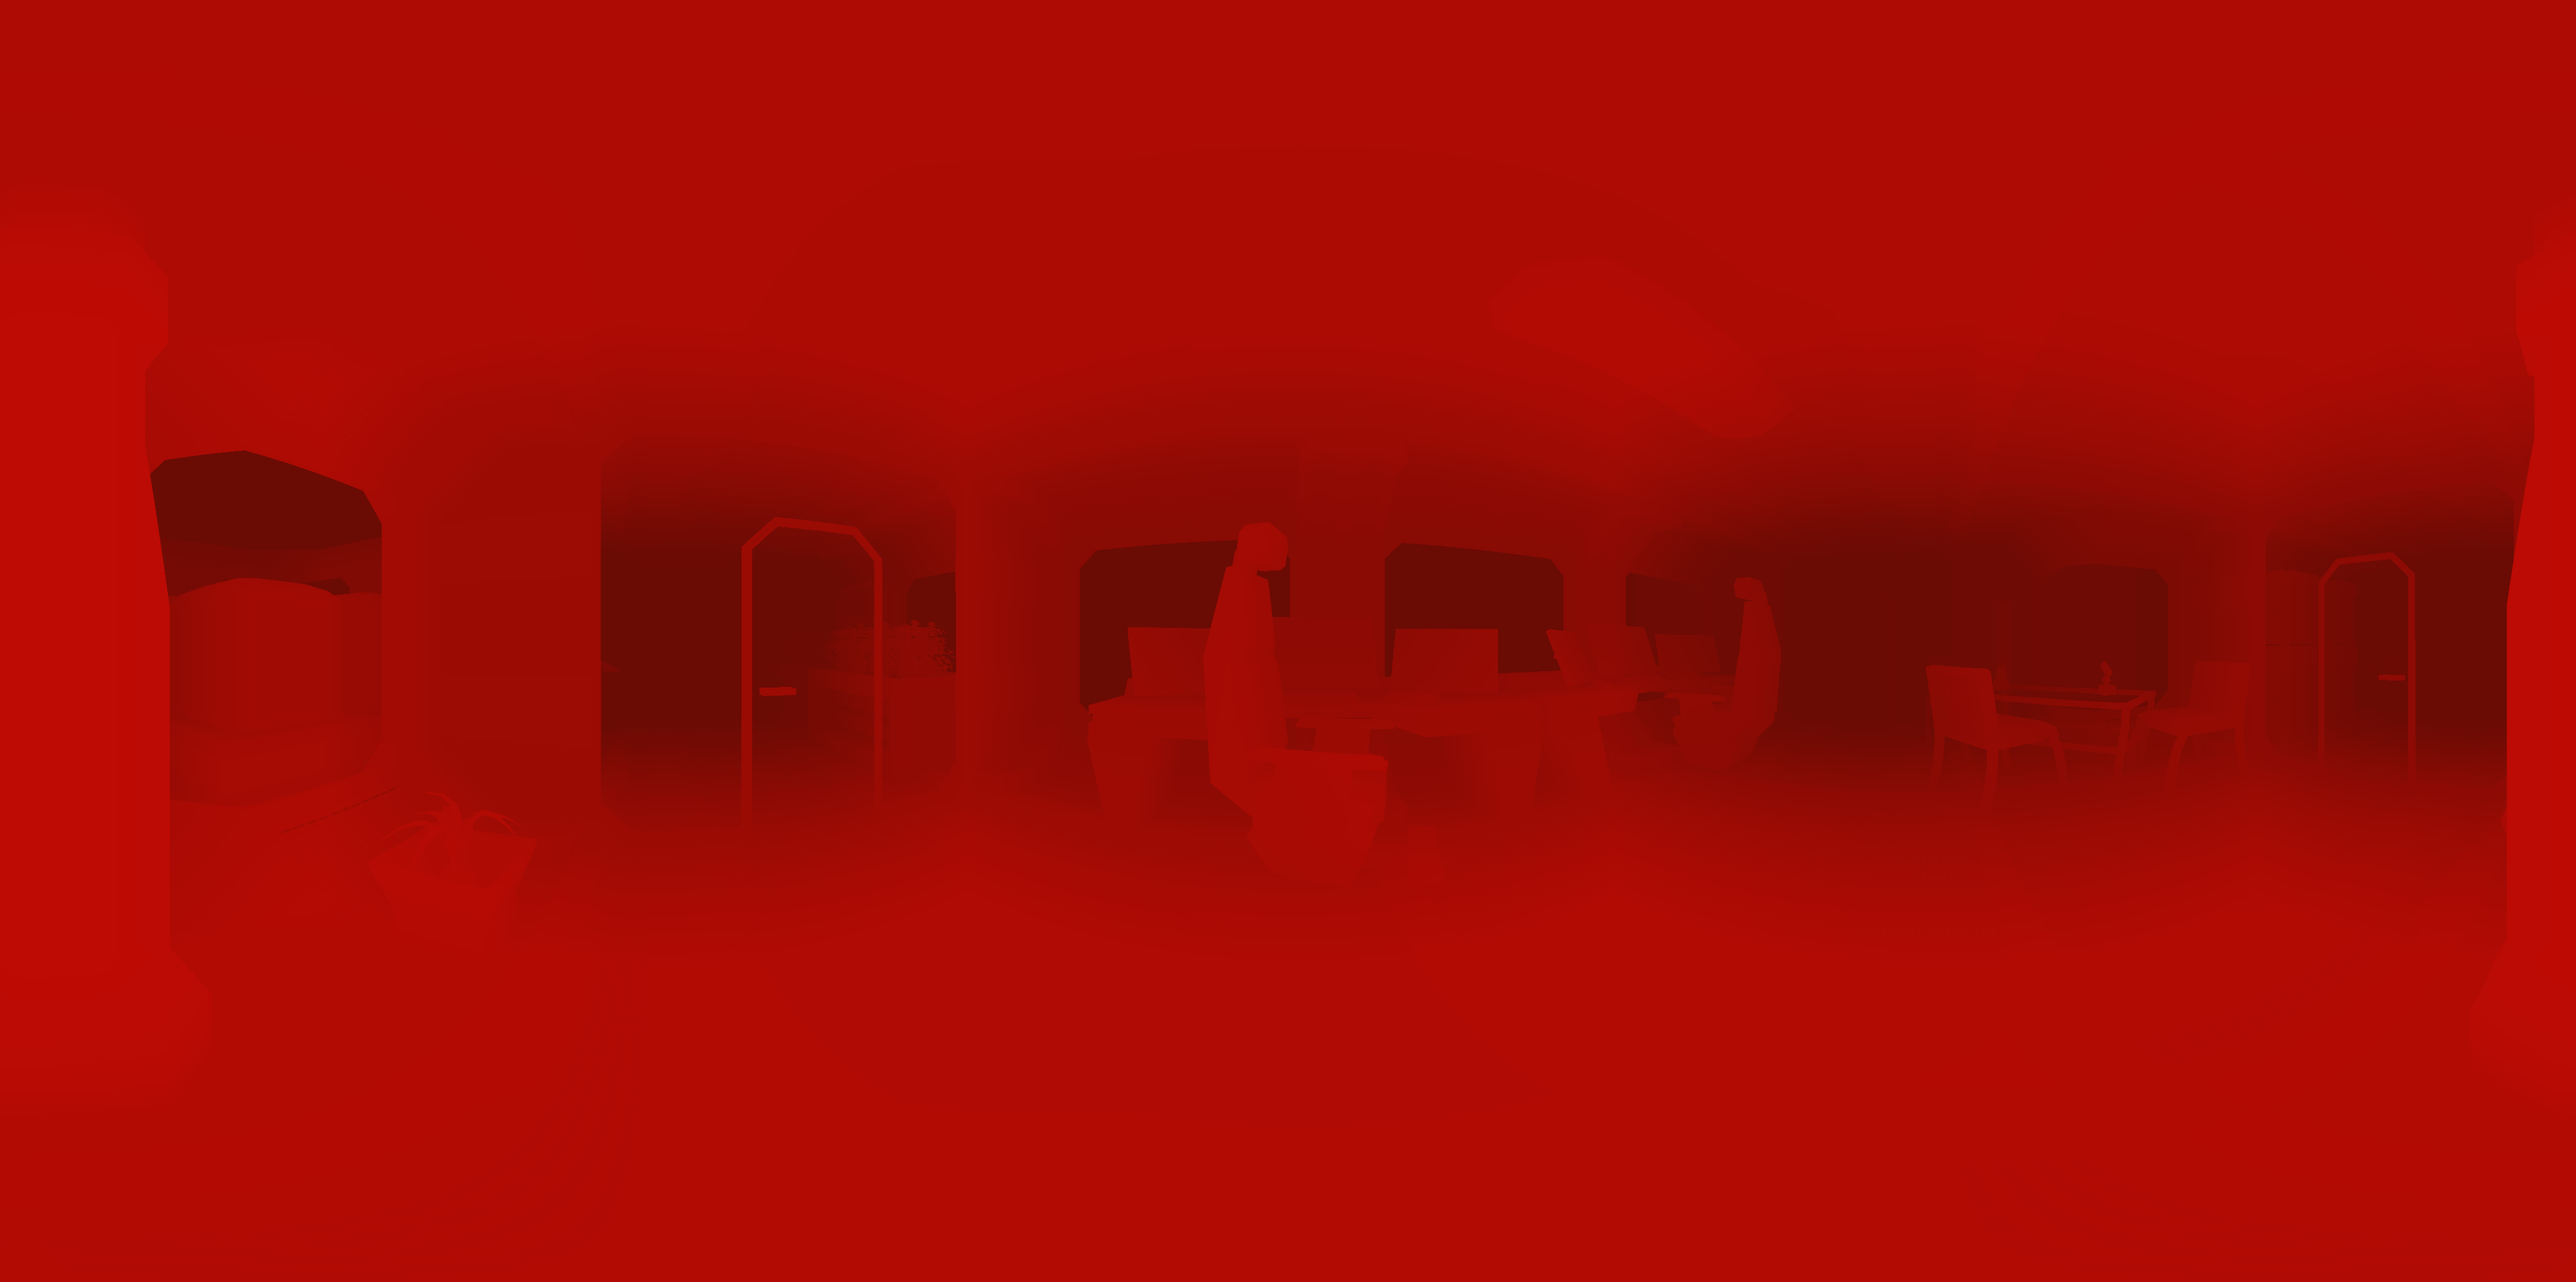
\includegraphics[width=0.8\textwidth]{red-depthmap-example}
  \caption{Ejemplo de mapa de profundidad 360 en escala de rojos}
  \label{fig:red-depthmap-example}
\end{figure}
\FloatBarrier

En el caso de la escala de grises (\ref{fig:depthmap-example}), los tonos más oscuros representan elementos en el fondo de la imagen, mientras que los tonos mas claro representan elementos más cercanos.

\begin{figure}[H]
  \centering
  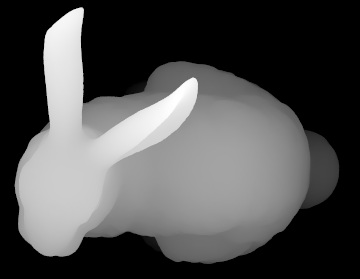
\includegraphics[width=0.6\textwidth]{depthmap-example}
  \caption{Ejemplo de mapa de profundidad cenital en escala de grises.}
  \label{fig:depthmap-example}
\end{figure}
\FloatBarrier

En el caso de una imagen generada por ordenador, es fácil obtener un buen mapa de profundidad. Sin embargo en el caso de las imágenes captadas por cámaras reales, existe la posibilidad de que la cámara esté preparada o en caso contrario habría que aplicar algoritmos que calculen la profundidad en cada píxel. 

Las cámaras que están preparadas para obtener el mapa de profundidad utilizan típicamente la emisión de infrarrojos. Existe una tecnología llamada LIDAR que obtiene mapas de profundidad de alta precisión con un haz láser, pero el tiempo que tarda en obtenerlo no lo hace compatible con la grabación de vídeo.

Dentro de los algoritmos que infieren el mapa de profundidad, los más conocidos utilizan imágenes estereoscópicas como el algoritmo BM  intenta parear elementos que se encuentren a la misma altura y el algoritmo SGBM que es una variación del anterior añadiendo una ventana de búsqueda para encontrar las correspondencias.

\subsection{Fotogrametría}
La fotogrametría consiste en deducir la ubicación de múltiples puntos en el espacio a partir de una serie de fotografías. Después de eso se reconstruyen los triángulos para generar una malla texturizada que represente de la manera más fiel posible la escena fotografiada. Javier de Matías analiza en profundidad la fotogrametría en \cite{PhotogrametryThesis}.

Al igual que en los mapas de profundidad, utilizar imágenes estereoscópicas ayudan a reconstruir la malla con mayor facilidad.

Algunos de los programas más conocidos para generación de mallas a partir de fotos son PIX4D y PhotoScan entre otros.


\section{Project Sidewinder}
Adobe presento en 2017 \cite{SidewinderAdobe} una demo que utilizaba un \textit{depthmap} de manera muy sencilla para permitir seis grados de libertad dentro de un video 360º. No proporcionan mucha información ya que es una prueba de concepto.

El desplazamiento punto a punto parece correcto pero se ve una distorsión en los bordes probablemente debido al estado temprano del proyecto.

\section{Nube de puntos}
Josh en \cite{Josh6DoFUnity} nos muestra una aplicación de esta técnica creando un punto en el espacio por cada píxel de la foto o el vídeo donde indique el mapa de profundidad.

\begin{figure}[H]
  \centering
  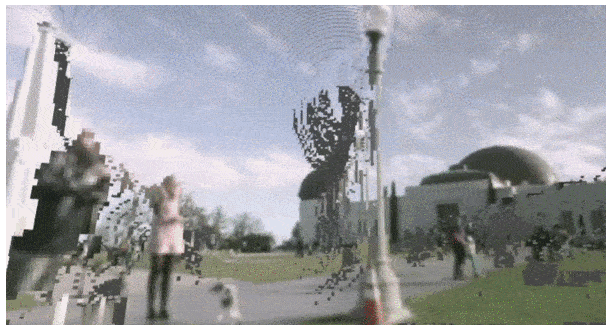
\includegraphics[width=0.8\textwidth]{pointcloud-example}
  \caption{Ejemplo de nube de puntos obtenida de \cite{Josh6DoFUnity}.}
  \label{fig:pointcloud-example}
\end{figure}
\FloatBarrier

Esta implementación por contra provoca que aparezcan muchos huecos como se puede ver en \ref{fig:depthmap-example} y generalmente se suele acompañar la implementación con una selección del tamaño del punto como muestra \cite{Josh6DoFUnity} para ver una imagen más sólida.

Otro de los problemas que tiene esta técnica es la cantidad de puntos que deben ser tratados, ya que una resolución \textit{QHD} (2560x1440) requiere cuatro millones de puntos siendo la resolución recomendada actualmente es \textit{4K}. Probablemente el rendimiento sea bajo en equipos poco potentes y en dispositivos móviles.

\section{Cámara y herramientas de realidad virtual de OTOY y Facebook}

En el F8 de 2017 en Los Ángeles \textit{OTOY} y \textit{Facebook} presentaron una colaboración para producir vídeo 360º volumétrico e interactivo a un precio asequible \cite{OtoyVR}. No hay noticias de 2018 por lo que puede que esté abandonado.

La colaboración consistía en una cámara 360º especializada y una serie de herramientas para procesar el contenido y visualizarlo. El procedimiento implica subir el contenido a la nube de OTOY para procesarlo y así reconstruir la escena como una malla tridimensional.

La calidad presentada en las demos era buena con poca distorsión aunque el desplazamiento que presentaban era pequeño.

\section{Facebook: Realidad virtual y Fotogrametría}
Una de las formas de conseguir seis grados de libertad es reconstruir la escena mediante fotogrametría como muestra \textit{Facebook} en \cite{FBCasual3DCapture} para procesar la imagen y obtener una malla que pueda ser mostrada usando técnicas convencionales.

\begin{figure}[H]
  \centering
	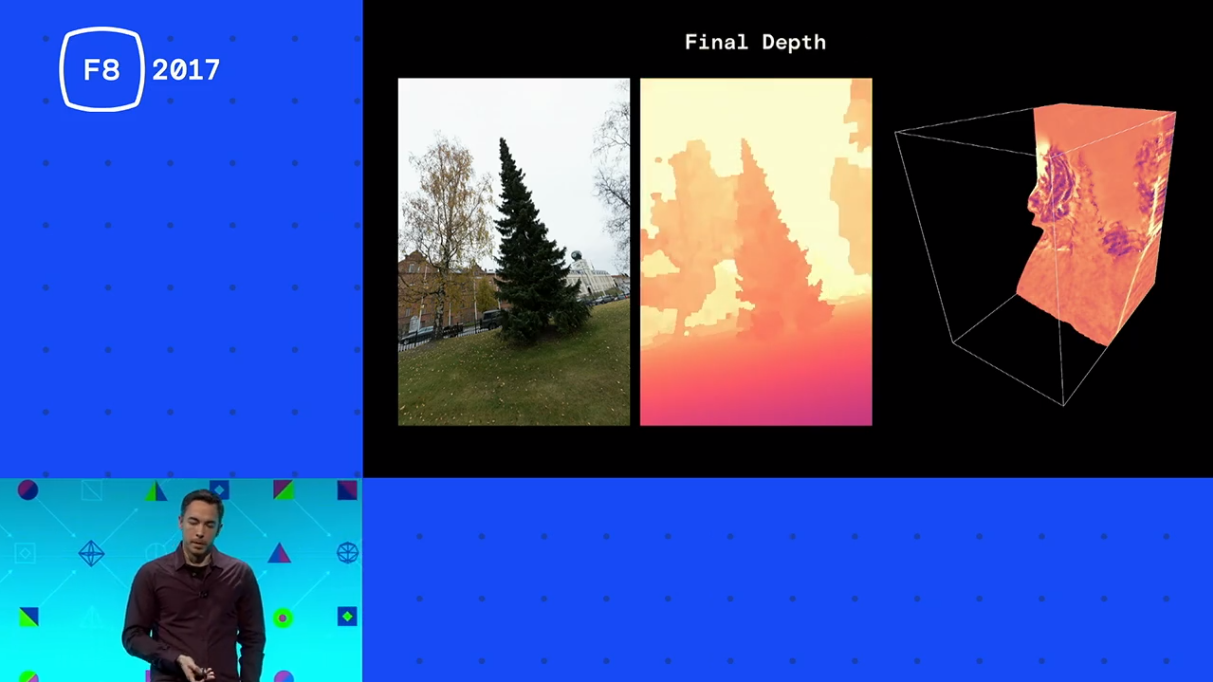
\includegraphics[width=\linewidth]{FB/fbdepthmap}
  \caption{Conferencia mostrando un mapa de profundidad de limite inferior obtenida de \cite{FBCasual3DCapture}.}
  \label{fig:fbLBdepthmap-example}
\end{figure}
\FloatBarrier

Este procedimiento utiliza una técnica nueva que han llamado ``mapa de profundidad de limite inferior'' (\ref{fig:depthmap-example}) que la profundidad de cada pixel debe ser estrictamente mayor que en el depthmap normal. Crear este mapa de profundidad le ayuda al ensamblado de las imágenes para crear la imágen final 360º. Además mezclando el mapa de profundidad con otros algoritmos son capaces de obtener un mapa de normales bastante preciso. \ref{fig:fbnormalmapcorrected-example}

\begin{figure}[H]
\centering
\begin{subfigure}{.47\linewidth}
	\centering
	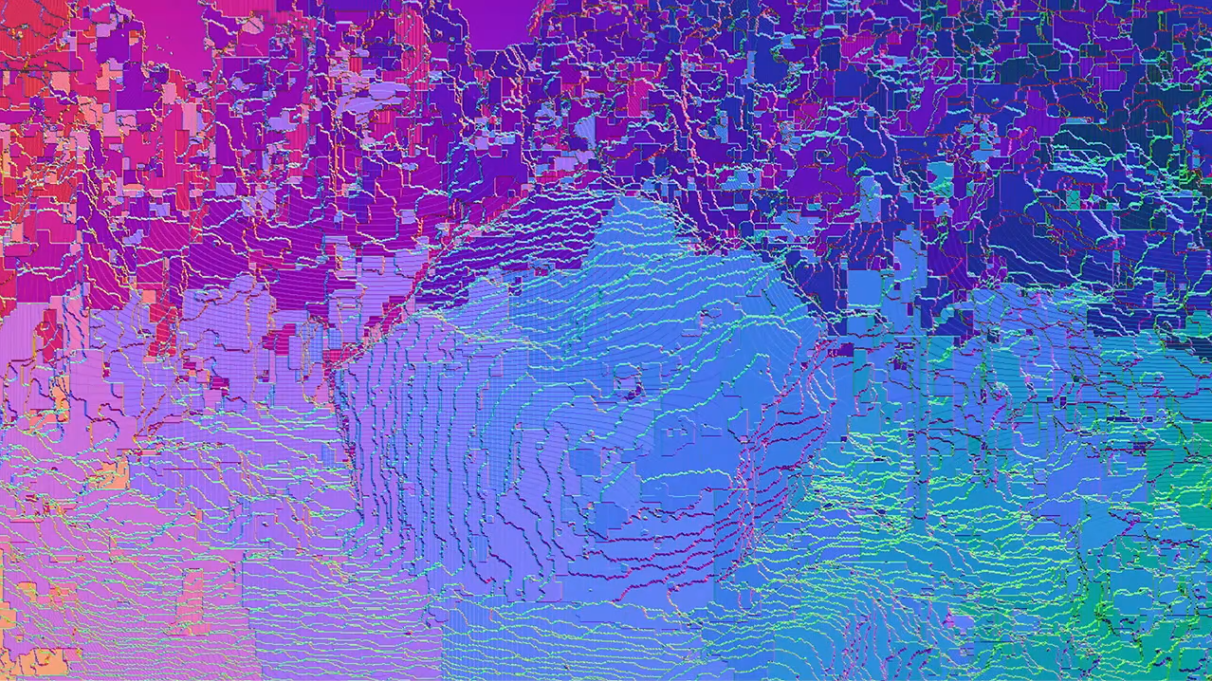
\includegraphics[width=\linewidth]{FB/fbnormalartifacts}
  \caption{Conferencia mostrando los artefactos que obtienen.}
  \label{fig:fbnormalmapartifacts-example}
\end{subfigure}%
\hspace{.05\linewidth}
\begin{subfigure}{.47\linewidth}
	\centering
	
\includegraphics[width=\linewidth]{FB/fbnormalmap}
  \caption{Conferencia mostrando los artefactos arreglados.}
  \label{fig:fbnormalmapcorrected-example}
\end{subfigure}
\caption{Imágenes obtenidas de \cite{FBCasual3DCapture}.}
\end{figure}
\FloatBarrier


Finalmente crean la malla a partir de una nube de puntos. Esta malla como veremos en otras técnicas, tiene agujeros detrás de los objetos que no pueden ser rellenados por falta de información. En este caso optan por difuminar de manera sutil las zonas desconocidas dando un buen resultado.

Todo esto lo aprovechan para poder generar un entorno tridimensional con el que poder interactuar y lo ejemplifican jugando con la iluminación \ref{fig:fblighting-example} o incluso inundando la escena \ref{fig:fbflooding-example}.

\begin{figure}[H]
\centering
\begin{subfigure}{.47\linewidth}
	\centering
	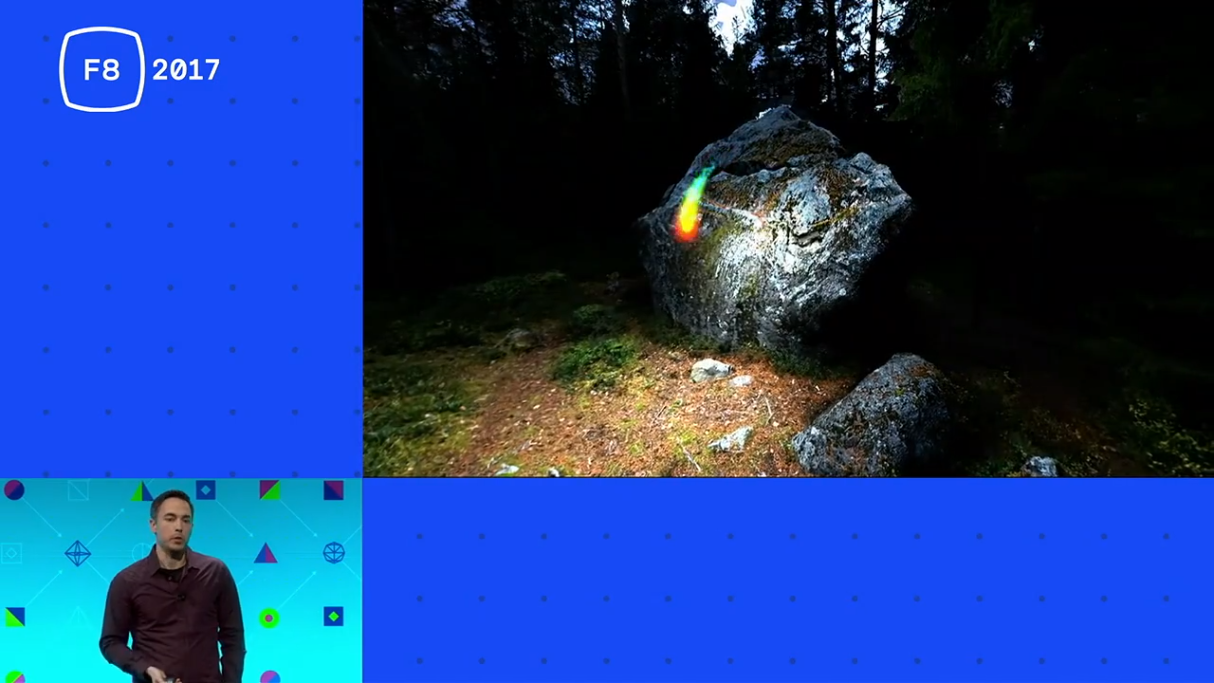
\includegraphics[width=\linewidth]{FB/fblighting}
  \caption{Conferencia mostrando la malla iluminada.}
  \label{fig:fblighting-example}
\end{subfigure}%
\hspace{.05\linewidth}
\begin{subfigure}{.47\linewidth}
	\centering
	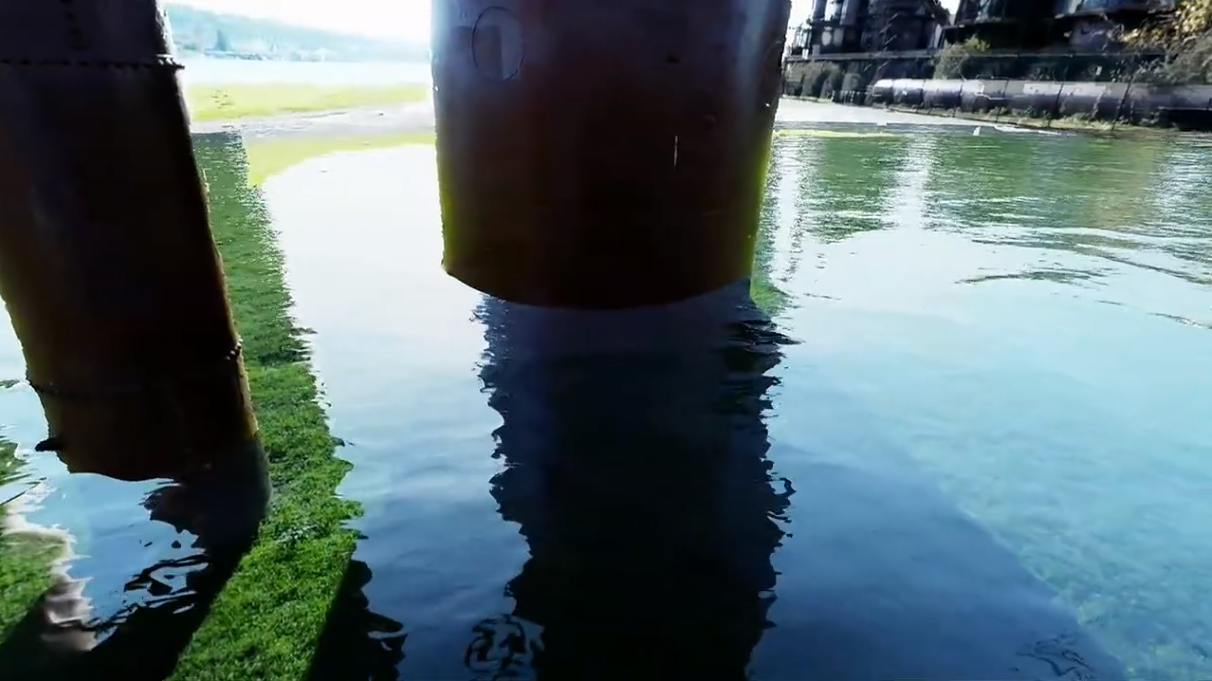
\includegraphics[width=\linewidth]{FB/fbflooding}
  \caption{Conferencia mostrando un escenario inundándose.}
  \label{fig:fbflooding-example}
\end{subfigure}
\caption{Imágenes obtenidas de \cite{FBCasual3DCapture}.}
\end{figure}
\FloatBarrier

Una de las limitaciones que tiene este método es que está diseñado para fotografía en 360º y no se menciona en ningún momento al vídeo 360º por lo que se puede deducir que no está preparado. Por otro lado este tipo de procesado de imágenes requiere una cantidad grande de tiempo.

\section{``Welcome to Lightfields''}
Una compañía llamada Lytro creo un sistema que llamo campos de luz o Lightfields \cite{LytroLightfields} por su similitud con el concepto físico. Más tarde Google se interesó por la compañía comprando algunas de sus patentes e incorporando empleados a su plantilla.

\textit{Google} continuó el proyecto \cite{GoogleLightfields} y construyó un soporte que permite hacer fotografías de una escena desde puntos situados en una esfera.

\begin{figure}[H]
  \centering
	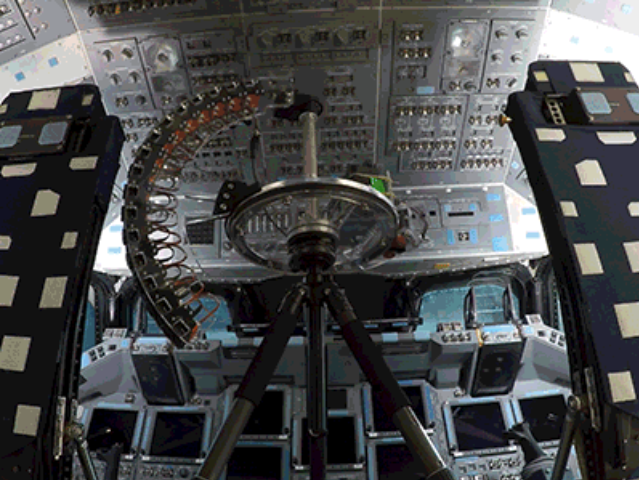
\includegraphics[width=0.8\linewidth]{lightfields-camera}
  \caption{Prototipo haciendo una captura del interior de una cabina. Obtenida de \cite{GoogleLightfields}.}
  \label{fig:lightfields-camera}
\end{figure}
\FloatBarrier

Este sistema no comprime las imágenes, sino que las utiliza directamente en el programa por lo que una ``foto'' en lightfields ocupa más de 250MB. A partir de todas las fotos se calcula la imagen correspondiente en tiempo real en función de la posición del usuario haciendo una interpolación entre diferentes imágenes, eso hace que se recupere una imagen muy fiel a lo que se vería en la realidad.

Como se puede apreciar en \ref{fig:lightfields-schema}, el usuario debe estar dentro de la esfera de fotos, por lo que el rango de movimiento está limitado a menos de un metro.

\begin{figure}[H]
  \centering
	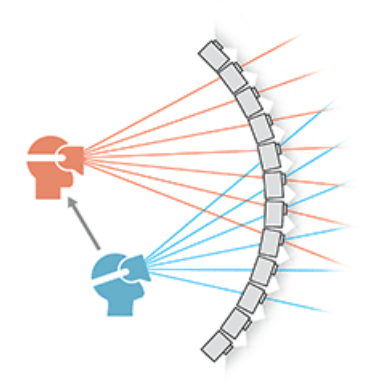
\includegraphics[width=0.5\linewidth]{lightfields-schema}
  \caption{Esquema de funcionamiento de los lightfields. Obtenida de \cite{GoogleLightfields}.}
  \label{fig:lightfields-schema}
\end{figure}
\FloatBarrier

Además este sistema tiene una implicación que no había sido contemplada hasta ahora que son las superficies especulares. Estas superficies en el resto de técnicas se podían ver con reflejo o no, pero nunca respondería a la posición del usuario. La interpolación de imágenes hace que los espejos reflejen algo diferente en cada posición de la cabeza.

Esta técnica para fotografía es probablemente la mejor en cuanto a calidad de imagen pero sin embargo no se puede utilizar en vídeo debido al tiempo que se tarda en capturar un sólo fotograma. Tampoco permite alterar la luz como se mostraba en la demo de \textit{Facebook}.













%DESARROLLO (40-45 hojas)
%----------------------------------------------------------------------------------------
%	DESARROLLO (40-45 hojas)
%----------------------------------------------------------------------------------------

\pagestyle{empty}
\chapter {Desarrollo}























%RESULTADOS (5-10 hojas)
%----------------------------------------------------------------------------------------
%	RESULTADOS (5-10 hojas)
%----------------------------------------------------------------------------------------

\pagestyle{empty}
\chapter {Resultados}

Los resultados visuales de los diferentes algoritmos se han ido comentando sobre la marcha en el apartado de Desarrollo, aquí se van a comentar

%CONCLUSIONES (2 hojas)
%----------------------------------------------------------------------------------------
%	CONCLUSIONES (2 hojas)
%----------------------------------------------------------------------------------------

\pagestyle{empty}
\chapter {Conclusiones}

El vídeo y la fotografía es hoy en día una parte imprescindible del entretenimiento en  realidad virtual. 

Sin embargo, tanto el vídeo como la fotografía son modelos de entretenimiento muy pobres en comparación con las experiencias interactivas que se ofrecen utilizando modelos tridimensionales. Por todo esto es importante preocuparse por mejorar estos medios y trabajar por ofrecer mejores soluciones.

Durante este proyecto se han estado trabajando con soluciones que hacen uso de algoritmos con una gran carga de trabajo, con su consecuente pérdida de rendimiento en los dispositivos de menores especificaciones. Para poder encontrar el algoritmo que mejor funciona hay que probar muchas implementaciones e ir descartando las soluciones menos prácticas.

Durante el desarrollo de las diferentes aproximaciones, encontré una serie de problemas a los que tuve que dar solución. Por ejemplo, utilizar un shader gráfico no era una opción viable para el programa.

Por otro lado, el código tiene partes donde se encontraron problemas que habitualmente se resuelven depurándolos, como es el caso de la función de desplazamiento en espacio de mundo. La depuración de shaders que se ejecutan sobre hardware gráfico es muy complicada de llevar a cabo y generalmente debe ser resuelta sacando colores por pantalla, cosa que no siempre es todo lo intuitivo que cabría esperar.

El objetivo propuesto tiene mucho fondo, pues el último propósito no estaba planteado para conseguirlo en el plazo de un trabajo de fin de máster, sino que todavía queda mucho trabajo por hacer en este campo. Aún así creo que se ha conseguido realizar una aproximación que permita continuar el desarrollo con nuevas características como el rellenado de huecos mediante imágenes que se encuentren paralelas a la actual y la sustitución de la vista actual por estas imágenes si el desplazamiento es superior a cierta cantidad.

Este trabajo a su vez ha requerido un gran componente de investigación, pues hay muchas y grandes empresas como Disney, Facebook y Google trabajando para hacer posible esta idea. Al ser empresas punteras en tecnología, lo hace un campo de trabajo muy complicado.

Como resultado de este trabajo puedo decir que las tecnologías de video e imagen en realidad virtual tienen mucho camino por recorrer pero que están encaminadas para que los creadores de contenido tengan una vía más completa de realizar sus obras.

Todavía queda mucho por hacer pero creo que no está muy lejos el día que, mientras tenemos unas gafas de realidad virtual puestas, podamos movernos alrededor de los personajes de nuestra película favorita y podamos sentirnos parte de ella.






\end{document}
